\documentclass[12pt]{report}
\usepackage[utf8]{inputenc}
\usepackage[english, russian]{babel}
\usepackage{listings}
\usepackage{graphicx}
\usepackage{float}
\graphicspath{{imgs/}}
\usepackage{amsmath,amsfonts,amssymb,amsthm,mathtools} 
\usepackage{pgfplots}
\usepackage{filecontents}
\usepackage{indentfirst}
\usepackage{eucal}
\usepackage{enumitem}
\frenchspacing

\usepackage{indentfirst} % Красная строка

\usetikzlibrary{datavisualization}
\usetikzlibrary{datavisualization.formats.functions}

\usepackage{amsmath}
\usepackage{fixltx2e}
\usepackage{caption}


\definecolor{bluekeywords}{rgb}{0,0,1}
\definecolor{greencomments}{rgb}{0,0.5,0}
\definecolor{redstrings}{rgb}{0.64,0.08,0.08}
\definecolor{xmlcomments}{rgb}{0.5,0.5,0.5}
\definecolor{types}{rgb}{0.17,0.57,0.68}

\usepackage{listings}
\lstset{language=[Sharp]C,
	captionpos=t,
	numbers=left, %Nummerierung
	numberstyle=\small, % kleine Zeilennummern
	frame=single, % Oberhalb und unterhalb des Listings ist eine Linie
	stepnumber=1,                   
	numbersep=5pt,                
	showspaces=false,
	tabsize=2,
	showtabs=false,
	breaklines=true,
	showstringspaces=false,
	breakatwhitespace=true,
	escapeinside={(*@}{@*)},
	commentstyle=\color{greencomments},
	morekeywords={partial, var, value, get, set},
	keywordstyle=\color{bluekeywords},
	stringstyle=\color{redstrings},
	basicstyle=\ttfamily\small,
}

\usepackage[left=2cm,right=2cm,top=1cm,bottom=2cm,bindingoffset=0cm]{geometry}
% Для измененных титулов глав:
\usepackage{titlesec, blindtext, color} % подключаем нужные пакеты
\definecolor{gray75}{gray}{0.75} % определяем цвет
\newcommand{\hsp}{\hspace{20pt}} % длина линии в 20pt
% titleformat определяет стиль
\titleformat{\chapter}[hang]{\Huge\bfseries}{\thechapter\hsp\textcolor{gray75}{|}\hsp}{0pt}{\Huge\bfseries}

\usepackage{array}
\newcommand{\head}[2]{\multicolumn{1}{>{\centering\arraybackslash}p{#1}}{#2}}

% plot
\usepackage{pgfplots}
\usepackage{filecontents}
\usetikzlibrary{datavisualization}
\usetikzlibrary{datavisualization.formats.functions}

\begin{document}
	%\def\chaptername{} % убирает "Глава"
	\thispagestyle{empty}
	\begin{titlepage}
		\noindent \begin{minipage}{0.15\textwidth}
			
\includegraphics[width=\linewidth]{b_logo}
		\end{minipage}
		\noindent\begin{minipage}{0.9\textwidth}\centering
			\textbf{Министерство науки и высшего образования Российской Федерации}\\
			\textbf{Федеральное государственное бюджетное образовательное учреждение высшего образования}\\
			\textbf{~~~«Московский государственный технический университет имени Н.Э.~Баумана}\\
			\textbf{(национальный исследовательский университет)»}\\
			\textbf{(МГТУ им. Н.Э.~Баумана)}
		\end{minipage}
		
		\noindent\rule{18cm}{3pt}
		\newline\newline
		\noindent ФАКУЛЬТЕТ $\underline{~~~~~~~~~~~~~~~~~~~\text{«Информатика, искусственный интеллект и системы управления»}~~~~~~~~~~~~~~~~~~~~~~~~~~~~~~~~~~~~~}$ \newline\newline
		\noindent КАФЕДРА $\underline{~~~~~~~~~~~~~\text{«Программное обеспечение ЭВМ и информационные технологии»}~~~~~~~~~~~~~~~~~~~~~~~}$\newline\newline\newline\newline\newline\newline\newline\newline\newline
		
		
		\begin{center}
			\noindent\begin{minipage}{1.3\textwidth}\centering
				\Large\textbf{  Отчет по лабораторной работе №3}\newline
				\textbf{по дисциплине \newline "Экономика программной инженерии"}\newline\newline
			\end{minipage}
		\end{center}
		
		\noindent\textbf{Тема} $\underline{\text{Оптимизация параметров проекта. Выравнивание загрузки ресурсов. Учет периодических}}$\newline\newline
		\indent\indent $\underline{\text{задач. Минимизация критического пути}}$\newline\newline
		\noindent\textbf{Студент} $\underline{\text{Малышев И. А.}}$\newline\newline
		\noindent\textbf{Группа} $\underline{\text{ИУ7-81Б}}$\newline\newline
		\noindent\textbf{Оценка (баллы)} $\underline{\text{~~~~~~~~~~~~~~~~~~~~~~~~~~~}}$\newline\newline
		\noindent\textbf{Преподаватель: } $\underline{\text{Барышникова М. Ю.}}$\newline\newline\newline
		
		\begin{center}
			\vfill
			Москва~---~\the\year
			~г.
		\end{center}
	\end{titlepage}
	
	\setcounter{page}{2}
	
	\chapter{Лабораторная работа}

\section{Цель работы}

Лабораторная работа № 2 выполняется на основе лабораторной работы № 1 и нацелена на освоение возможностей программы Microsoft Project для работы с ресурсами.

\section{Содержание проекта}

Команда разработчиков из 16 человек занимается созданием карты города на основе собственного модуля отображения. Проект должен быть завершен в течение 6 месяцев. Бюджет проекта: 50 000 рублей.

\section{Задание 1: Создание списка ресурсов}

Был заполнен ресурсный лист в соответствии с таблицей.

\begin{figure}[H]
	\begin{center}
		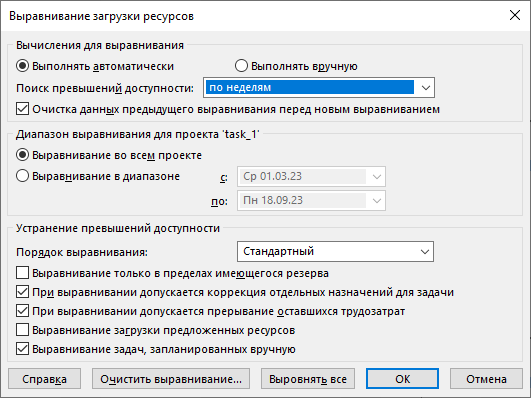
\includegraphics[width=\textwidth]{imgs/task_1_0.png}
	\end{center}
\end{figure}

\section{Задание 2: Назначение ресурсов задачам}

Было установлено соответствие исполнителям зачач, добавлены фиксированные затраты.

\begin{figure}[H]
	\begin{center}
		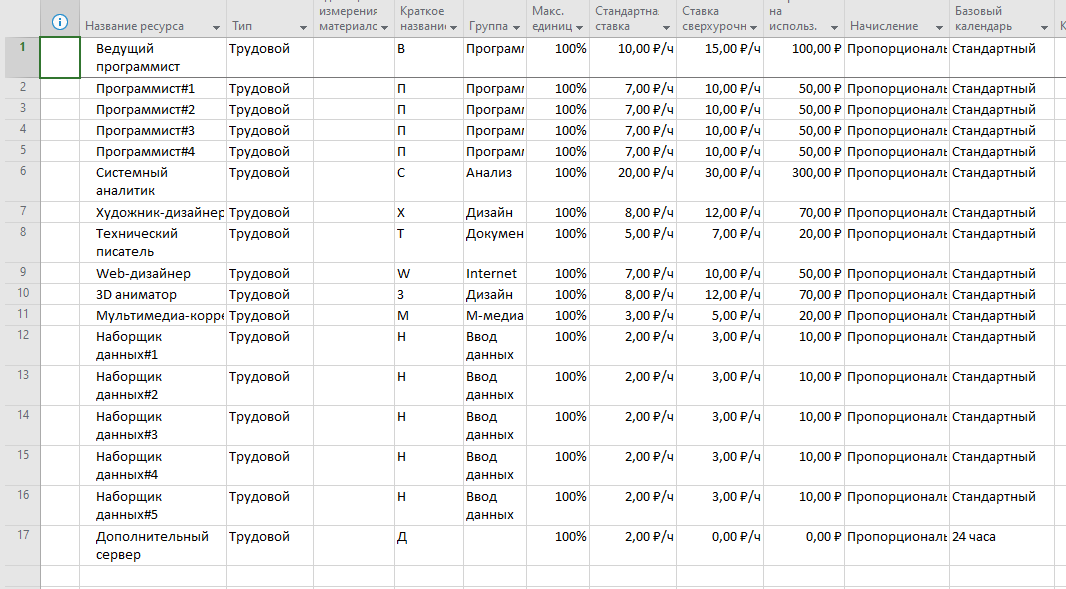
\includegraphics[width=\textwidth]{imgs/task_1_1.png}
	\end{center}
\end{figure}

У исполнителей появились перегрузки из-за того, что они заняты на нескольких задачах одновременно. Продемонстрируем это на оптимизаторе ресурсов:

\begin{figure}[H]
	\begin{center}
		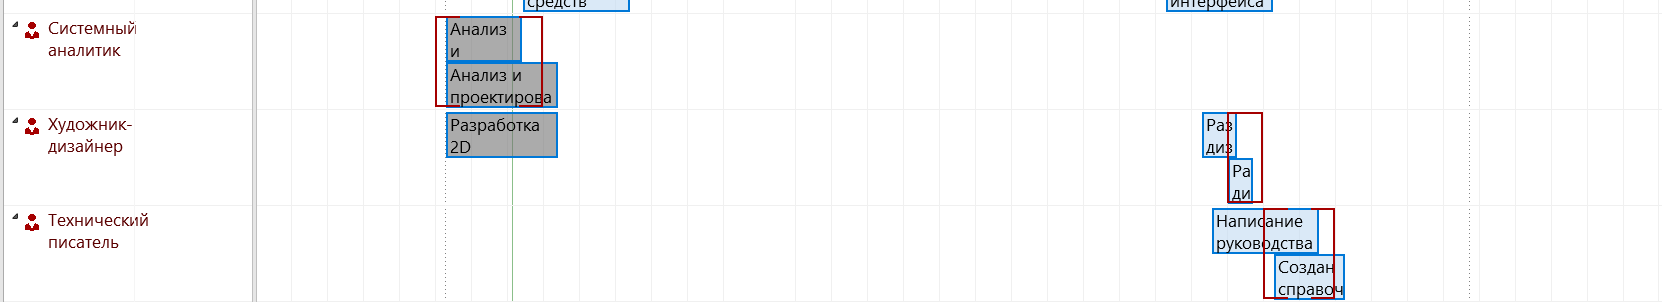
\includegraphics[width=\textwidth]{imgs/task_1_2.png}
	\end{center}
\end{figure}

\begin{figure}[H]
	\begin{center}
		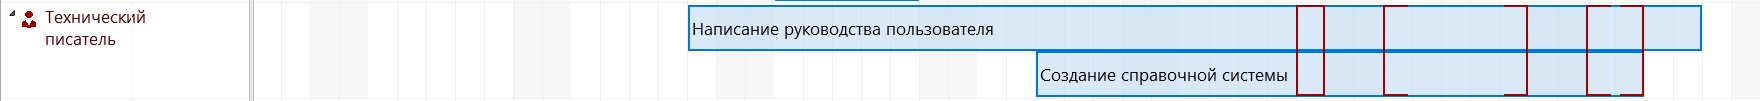
\includegraphics[width=\textwidth]{imgs/task_1_2_1.png}
	\end{center}
\end{figure}

Результаты:

\begin{figure}[H]
	\begin{center}
		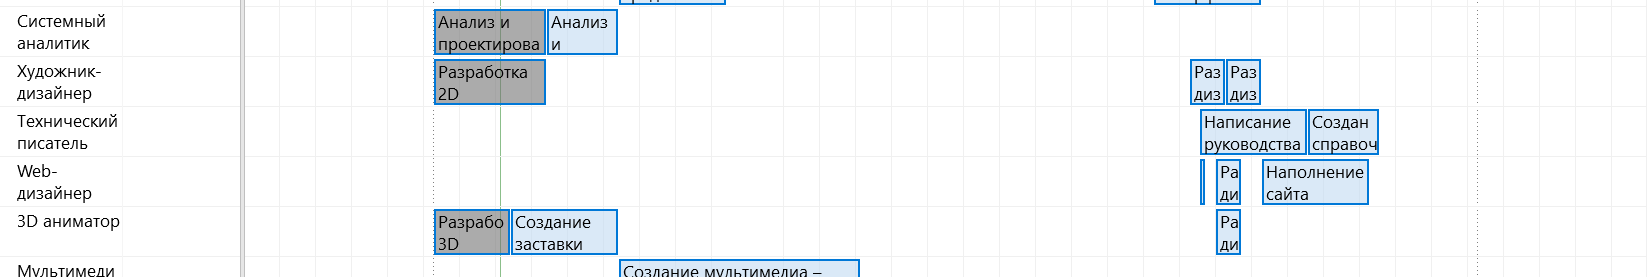
\includegraphics[width=\textwidth]{imgs/task_1_3.png}
	\end{center}
\end{figure}

\begin{figure}[H]
	\begin{center}
		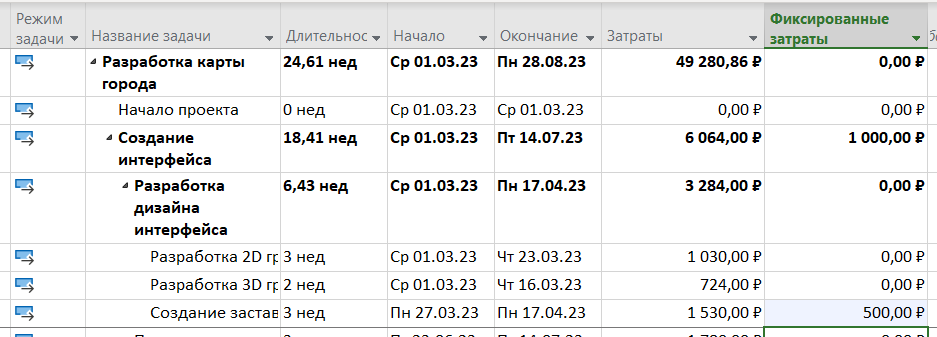
\includegraphics[width=\textwidth]{imgs/task_1_4.png}
	\end{center}
\end{figure}

\begin{figure}[H]
	\begin{center}
		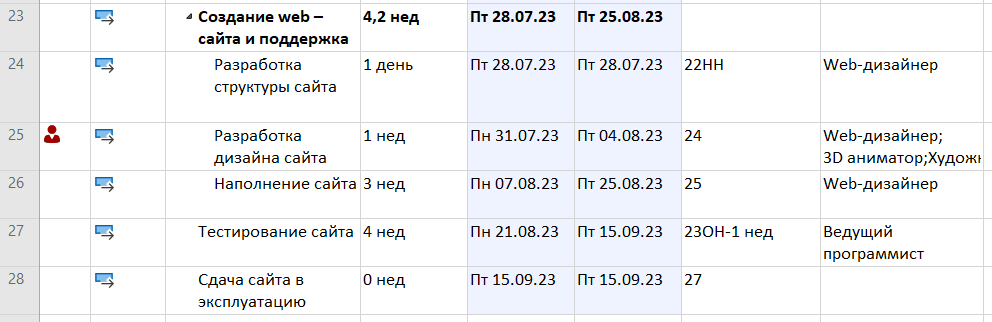
\includegraphics[width=\textwidth]{imgs/task_1_5.png}
	\end{center}
\end{figure}

\section{Задание 3: Анализ затрат по группам ресурсов}

Было просмотренно использование ресурсов, данные сгрупированны по группам.

\begin{figure}[H]
	\begin{center}
		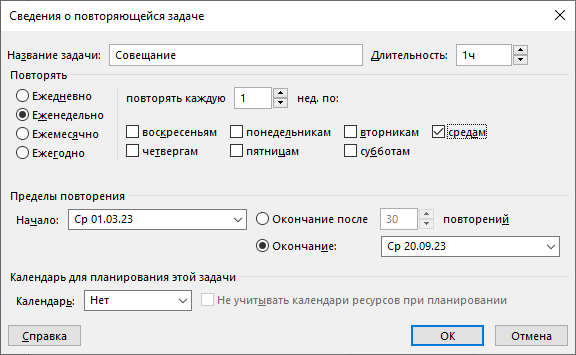
\includegraphics[width=\textwidth]{imgs/task_2_0.png}
	\end{center}
\end{figure}

Вручную было построено два графика:

\begin{figure}[H]
	\begin{center}
		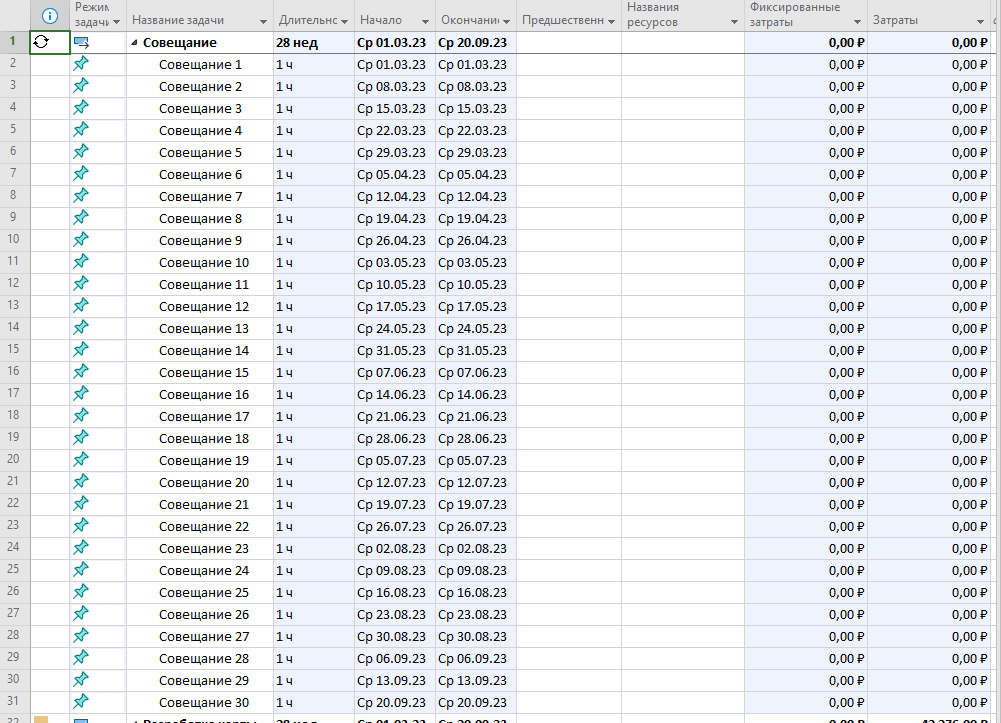
\includegraphics[width=\textwidth]{imgs/task_2_1.png}
	\end{center}
\end{figure}

\begin{figure}[H]
	\begin{center}
		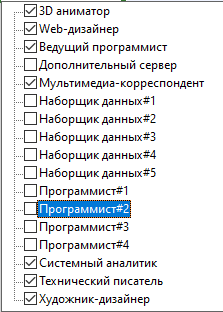
\includegraphics[width=\textwidth]{imgs/task_2_2.png}
	\end{center}
\end{figure}

\textbf{Выводы}

Происходит перегруженность сотрудников, следует решить эту задачу.

Наборщики данных, выполняя 26 \% работы, получают к оплате 11 \% бюджета. Аналитик при всего 2 \% трудозатрат требует 10 \% от всего бюджета. Программисты, выполняя 29 \% работ, требует 50 \% бюджета. Требуется оптимизация ресурсов.
	
	\chapter{Выводы}

В результате выполнения лабораторной работы был разработан программный инструмент для оценки проекта по методике COCOMO. Были изучены существующие методики предварительной оценки параметров программного проекта, а также проведена практическая оценка затрат проекта.

По результатам применения методики оценки COCOMO можно заключить, что она пригодна для общей предварительной оценки всего проекта и позволяет получить приблизительные значения трудозатрат и времени на реализацию проекта, разделенные на стадии его жизненного цикла. Однако для постоянного отслеживания состояния проекта рекомендуется использовать другие методики управления проектами с использованием различных программных средств, которые позволяют актуализировать данные проекта в реальном времени и своевременно адаптироваться к непредвиденным изменениям в проекте.
	
\end{document}